\documentclass[2pt,a4paper]{article}
\usepackage{tikz}
\usetikzlibrary{shapes,positioning,calc}
\colorlet{lightgray}{gray!20}

\begin{document}

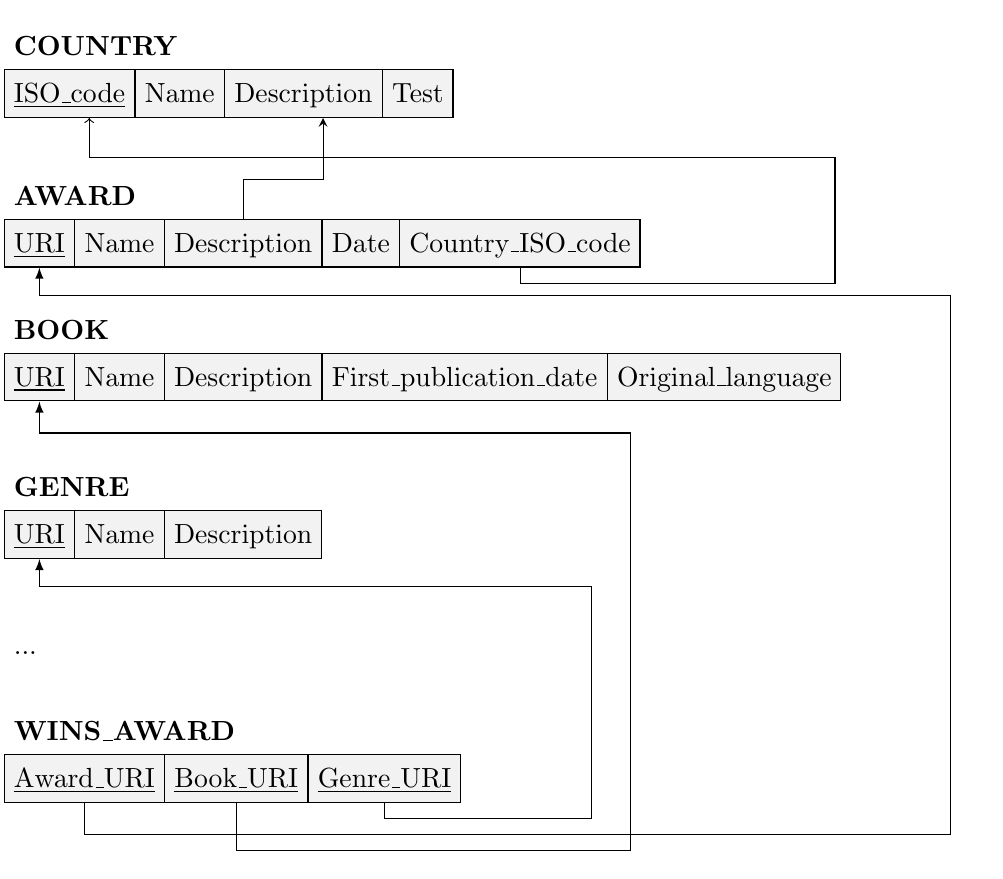
\begin{tikzpicture}[relation/.style={rectangle split, rectangle split parts=#1, rectangle split part align=base, draw, anchor=center, align=center, text height=3mm, text centered}]\hspace*{-0.3cm}

% RELATIONS

\node (countrytitle) {\textbf{COUNTRY}};

\node [relation=4, rectangle split horizontal, rectangle split part fill={lightgray!50}, anchor=north west, below=0.6cm of countrytitle.west, anchor=west] (country)
{\underline{ISO\_code}%
\nodepart{two}   Name
\nodepart{three} Description
\nodepart{four} Test};

\node [below=1.3cm of country.west, anchor=west] (awardtitle) {\textbf{AWARD}};

\node [relation=5, rectangle split horizontal, rectangle split part fill={lightgray!50}, below=0.6cm of awardtitle.west, anchor=west] (award)
{\underline{URI}%
\nodepart{two} Name
\nodepart{three} Description
\nodepart{four}  Date
\nodepart{five}  Country\_ISO\_code};

\node [below=1.1cm of award.west, anchor=west] (booktitle) {\textbf{BOOK}};

\node [relation=5, rectangle split horizontal, rectangle split part fill={lightgray!50}, anchor=north west, below=0.6cm of booktitle.west, anchor=west] (book)
{\underline{URI}%
\nodepart{two}   Name
\nodepart{three} Description
\nodepart{four}  First\_publication\_date
\nodepart{five} Original\_language};

\node [below=1.4cm of book.west, anchor=west] (genretitle) {\textbf{GENRE}};

\node [relation=3, rectangle split horizontal, rectangle split part fill={lightgray!50}, anchor=north west, below=0.6cm of genretitle.west, anchor=west] (genre)
{\underline{URI}%
\nodepart{two}   Name
\nodepart{three} Description};

\node [below=1.5cm of genre.west, anchor=west] (ell1) {...};

\node [below=1.0cm of ell1.west, anchor=west] (winsawardtitle) {\textbf{WINS\_AWARD}};

\node [relation=3, rectangle split horizontal, rectangle split part fill={lightgray!50}, anchor=north west, below=0.6cm of winsawardtitle.west, anchor=west] (winsaward)
{\underline{Award\_URI}%
\nodepart{two}   \underline{Book\_URI}
\nodepart{three} \underline{Genre\_URI}};

% FOREIGN KEYS

\draw[->] (award.five south) -- ++(0,-0.2) -| ($(award.five south) + (4,0)$) |- ($(country.one south) + (0.25,-0.50)$) -| ($(country.one south) + (0.25,0)$);

%\draw[-latex] (award.three north) |- ($(country.three south) + (0.25,-0.75)$) -| ($(country.three south) + (0.25,0)$) ;

\draw[-stealth] (award.three north) -- ++(0,0.5) -|  ($(country.three south) + (0.25,0)$) ;


\draw[-latex] (winsaward.one south) -- ++(0,-0.4) -| ($(winsaward.one south) + (11,0)$) |- ($(award.one south) + (0,-0.35)$) -| ($(award.one south) + (0,0)$);

\draw[-latex] ($(winsaward.two south) + (0.00,0)$) |- ++(0,-0.60) -| ($(winsaward.two south) + (5,0)$) |- ($(book.one south) + (0.00,-0.40)$) -| ($(book.one south) + (0.00,0)$);

\draw[-latex] (winsaward.three south) -- ++(0,-0.2) -| ($(winsaward.three south) + (2.63,0)$) |- ($(genre.one south) + (-0.00,-0.35)$) -| ($(genre.one south) + (-0.0,0)$);

\end{tikzpicture}

\end{document}